\documentclass[10pt]{article}
% Executive summary: Is Selling S&P 500 Volatility a Free Lunch?
% Compiles with pdflatex (or on Overleaf). No external files needed.

\usepackage[letterpaper,hmargin=0.7in,vmargin=0.55in]{geometry}
\usepackage[T1]{fontenc}
\usepackage{charter}
\usepackage[scaled=0.9]{helvet}
\usepackage{amsmath}
\usepackage{booktabs}
\usepackage{tabularx}
\usepackage{array}
\usepackage{enumitem}
\usepackage{xcolor}
\usepackage{pgfplots}
\pgfplotsset{compat=1.17}
\usepackage[hidelinks]{hyperref}
\usepackage{titlesec}

\definecolor{ink}{HTML}{14213D}
\definecolor{accent}{HTML}{2E6F95}
\definecolor{muted}{HTML}{7A8594}

\titleformat{\section}{\normalfont\large\bfseries\color{ink}}{}{0pt}{}
\titlespacing*{\section}{0pt}{6pt}{2pt}
\setlength{\parindent}{0pt}
\setlength{\parskip}{3pt}
\setlist{nosep,leftmargin=1.2em}
\renewcommand{\arraystretch}{1.15}

\begin{document}

\begin{center}
{\LARGE\bfseries\color{ink} Is Selling S\&P 500 Volatility a Free Lunch?}\\[4pt]
{\large Executive summary}\\[2pt]
Nahid Hasan Sagar \& Team\quad$\cdot$\quad Erd\H{o}s Institute Quant Finance Boot Camp, Fall 2026 \quad$\cdot$\quad November 5, 2026
\end{center}

\textbf{Answer in one line:} selling S\&P 500 volatility has paid on average since 2005, but it is not a free lunch. The payoff is payment for crash risk, it is only borderline significant once crashes are counted, and in real options the edge is thin.

\textbf{The question.} Investors buy S\&P 500 options as crash insurance. If option prices imply more volatility than the market then delivers, the sellers earn a \emph{variance risk premium}. We ask how large it is, how reliable it is, what it costs in crises, whether it can be timed, and whether it survives in real, hedged options.

\section*{Data and method}
5,495 trading days, January 2005 to November 2026: S\&P 500, VIX and VIX3M (Yahoo Finance) and the 3-month T-bill (FRED).
\begin{itemize}
  \item \textbf{The premium} is $\text{VRP}_t = \text{VIX}_t^2/10{,}000 - \tfrac{252}{21}\sum_{i=1}^{21} r_{t+i}^2$, where $r$ is the daily log return of the S\&P 500. It equals the profit of selling a one-month variance swap.
  \item \textbf{Inference.} Daily observations overlap by 20 of 21 days, so we use Newey--West standard errors (21--42 lags). We also run a t-test on non-overlapping months for all 21 possible start days, plus a sign test.
  \item \textbf{Forecasting and timing.} A HAR model, refit monthly on past data only, is scored against VIX$^2$ and last month's variance (MSE, QLIKE). A trading rule was committed to the repository before testing, trained on 2008--2015 and tested once on 2016 onwards.
  \item \textbf{Real options.} Each month we sell a 30-day at-the-money straddle priced at VIX minus 0--3 vol points and delta hedge it daily with Black--Scholes. We split its P\&L into theta and gamma, after checking the hedge on simulated GBM paths.
\end{itemize}

\section*{Finding 1: the premium is real, usually positive, and fragile}
VIX exceeded the volatility that followed on 84\% of days, by 3.5 vol points on average. On non-overlapping months, 82\% of months were profitable for the seller. A sign test rejects a 50/50 coin overwhelmingly (215 of 261 months, $p \approx 10^{-27}$).

The \emph{average} is far less certain. The Newey--West t-statistic is 2.1--2.3, and the non-overlapping t-statistic ranges from 1.6 to 2.6 depending on the start day. The payoff has skew $-5.4$ and excess kurtosis 42: one month, March 2020, erased about 46 typical months of gains. Most months win, and a few crashes decide the total.

\section*{Finding 2: crashes, not bear markets, hurt the seller}
A swap sold on the first day of every stress episode since 2008 lost money (Figure~\ref{fig:episodes}). In 2022 stocks fell about 25\%, but slowly, and VIX had priced the decline in advance. In August 2024 VIX jumped to 38.6 while realized volatility stayed near 19\%, so the seller barely lost.

\begin{figure}[!ht]
\centering
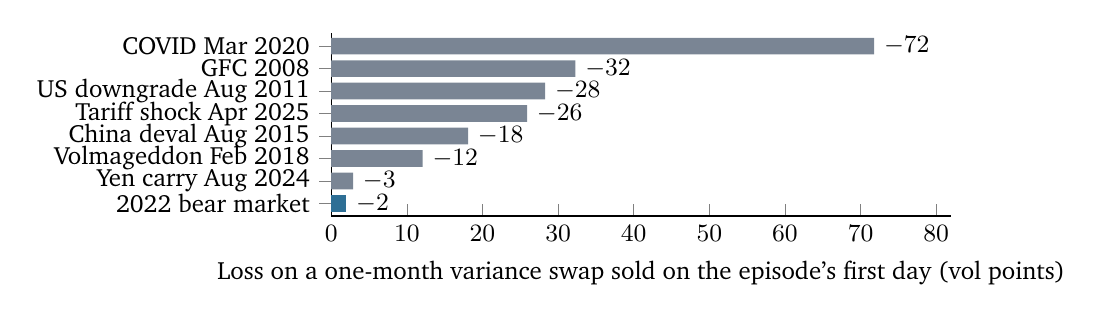
\begin{tikzpicture}
\begin{axis}[
  xbar, bar width=6pt, bar shift=0pt,
  width=0.78\linewidth, height=3.9cm,
  xmin=0, xmax=82,
  symbolic y coords={2022 bear market,Yen carry Aug 2024,Volmageddon Feb 2018,China deval Aug 2015,Tariff shock Apr 2025,US downgrade Aug 2011,GFC 2008,COVID Mar 2020},
  ytick={2022 bear market,Yen carry Aug 2024,Volmageddon Feb 2018,China deval Aug 2015,Tariff shock Apr 2025,US downgrade Aug 2011,GFC 2008,COVID Mar 2020}, y tick label style={font=\small},
  xlabel={Loss on a one-month variance swap sold on the episode's first day (vol points)},
  xlabel style={font=\small}, x tick label style={font=\small},
  axis x line*=bottom, axis y line*=left,
  nodes near coords={$-$\pgfmathprintnumber[fixed,precision=0]{\pgfplotspointmeta}},
  nodes near coords style={font=\small, anchor=west},
  enlarge y limits=0.08,
]
\addplot[fill=muted, draw=none] coordinates {
  (71.8,COVID Mar 2020) (32.3,GFC 2008) (28.3,US downgrade Aug 2011) (25.9,Tariff shock Apr 2025)
  (18.1,China deval Aug 2015) (12.1,Volmageddon Feb 2018) (2.9,Yen carry Aug 2024)};
\addplot[fill=accent, draw=none] coordinates {(2.0,2022 bear market)};
\end{axis}
\end{tikzpicture}
\caption{Sudden crashes cost the seller up to 72 vol points; the slow 2022 bear cost 2 (notebook 02).}
\label{fig:episodes}
\end{figure}

\section*{Finding 3: VIX is an accurate but overpriced forecast, and a simple filter cuts risk}
VIX$^2$ forecasts next-month variance better than HAR (QLIKE 0.37 vs 0.39, MSE 45 vs 58 $\times 10^{-4}$) even though it runs 0.008 too high on average. That bias is the premium itself. HAR clearly beats last month's variance (QLIKE 0.57), so the model works.

The rule sells only when the HAR forecast premium is positive and the VIX curve is not inverted. It is in the market about 56\% of months. In the 2016+ test it keeps the average gain (paired $t = 0.09$) and cuts risk:

\begin{center}
\begin{tabular}{lrr}
\toprule
Variance swap, test period 2016+ & Always sell & Rule \\
\midrule
Sharpe, median of 21 start days & 0.36 & 1.20 \\
Worst month, median of 21 start days & $-0.73$ & $-0.18$ \\
Worst month, unluckiest start day & $-0.82$ & $-0.80$ \\
\bottomrule
\end{tabular}
\end{center}

The last row is the catch: the rule was on when COVID began from calm markets. It avoids the second wave of a crash, not the first hit.

\section*{Finding 4: in real hedged options the edge survives, but it is thin}
A delta-hedged short straddle earns money only if it is sold close to VIX. VIX includes out-of-the-money puts, so at-the-money options trade a few points below it, and the realistic rows are the 2--3 point haircuts.

\begin{center}
\begin{tabular}{lrrrr}
\toprule
Straddle priced at & Mean P\&L / month & Sharpe (annual) & Months positive & Mean after option cost \\
\midrule
VIX              & $+0.77\%$ & 2.1 & 81\% & $+0.66\%$ \\
VIX $-$ 1 pt     & $+0.54\%$ & 1.5 & 76\% & $+0.43\%$ \\
VIX $-$ 2 pts    & $+0.32\%$ & 0.9 & 69\% & $+0.20\%$ \\
VIX $-$ 3 pts    & $+0.09\%$ & 0.3 & 59\% & $-0.02\%$ \\
\bottomrule
\end{tabular}
\end{center}

The hedge behaves as theory says. On simulated GBM paths, a straddle priced 2 points too high earns 0.47\% of the index against a predicted 0.46\%. On real data, summing the daily gamma--theta approximation $\tfrac12\,\Gamma_t S_t^2(\sigma_{\text{imp}}^2\,\Delta t - r_t^2)$ tracks the monthly P\&L with correlation 0.98: the trade earns theta when markets are calm and loses gamma when they move. Hedging softens the tail (skew $-0.8$ vs $-5.4$ for the swap), but the worst month is still March 2020 at $-5.8\%$. With the same filter at a 2-point haircut, the 2016+ Sharpe rises from 0.91 to 1.29 for the same mean.

\section*{Limitations}
\begin{center}
\small
\begin{tabularx}{\linewidth}{>{\raggedright\arraybackslash}X >{\raggedright\arraybackslash}p{0.2\linewidth} >{\raggedright\arraybackslash}X}
\toprule
Assumption & Likely effect & How we controlled for it \\
\midrule
Straddles priced at VIX, which includes out-of-the-money puts & Overstates the at-the-money premium & Haircuts of 0--3 vol points; we read the 2--3 point rows as realistic \\
Few independent crashes (three in the 2016+ test) & Tail and Sharpe estimates are noisy & Non-overlapping tests over all 21 start days; tail results reported, not just means \\
Costs: 0.5 vol point $\times$ vega on the option; no hedge costs, bid--ask, margin or dividends & Overstates net P\&L & Net-of-cost column; the edge is about zero at a 3-point haircut \\
Straddles enter on the first trading day of each month only & Results depend on the calendar & Start-day robustness shown for the variance swap; not yet repeated for straddles \\
Rule chosen with hindsight & Inflates out-of-sample results & Rule committed to the repository before testing; signal uses the previous close; HAR refit on past data only \\
\bottomrule
\end{tabularx}
\end{center}

\section*{Practical takeaway and what we learned}
For a portfolio manager, short volatility is insurance underwriting, not free money. Size it so that a March-2020 month is survivable: $-0.5$ variance units on a swap, or $-6\%$ of the index on a hedged straddle. A forecast-based filter roughly halves the tail without giving up return, but it cannot dodge a crash that starts from calm markets.
\begin{itemize}
  \item \textbf{Overlap matters.} Ignoring it inflates the t-statistic about four-fold (8.9 vs 2.3).
  \item \textbf{Heavy tails split mean and median:} the median month gains 0.011, the mean only 0.006.
  \item \textbf{Commit a rule before testing it.} It was the only way to make an out-of-sample claim we could defend.
\end{itemize}

\section*{Contributions and reproducibility}
\textbf{Nahid Hasan Sagar:} data pipeline, premium measurement and tests, crisis analysis, HAR forecast and trading rule, straddle backtest and attribution, write-up and video.
\textbf{Kevin:} initial GBM path simulation in notebook 04. % TODO: confirm or edit before submitting
\textbf{Anatolii Vakaryuk:} joined the team late, helped with some writing and editing, and provided feedback on the final report.

Code, data and notebooks are at \url{https://github.com/Sagar-DU/volatility-risk-premium}. To reproduce, install \texttt{requirements.txt} and run notebooks 01 $\to$ 04 in order. Data is pulled from Yahoo Finance and FRED, and \texttt{pytest} checks the core functions.

\end{document}
